\section{Discussion}
\label{sec:discussion}

\subsection{The Interpretive Process of Public Robot Sensemaking}
\label{sec:service-justification}
% Sensemaking is a process, not an immediate evaluation
% Encountering makes the robot interpretively salient
% Interpreting is organized around WHAT, HOW, and WHO
    % Participants construct answers from available cues and reasoning strategies
% Situating turns an interpretation into a judgment about the robot’s place
% Imply and connect to local legibility

\begin{figure*}[t]
    \centering
    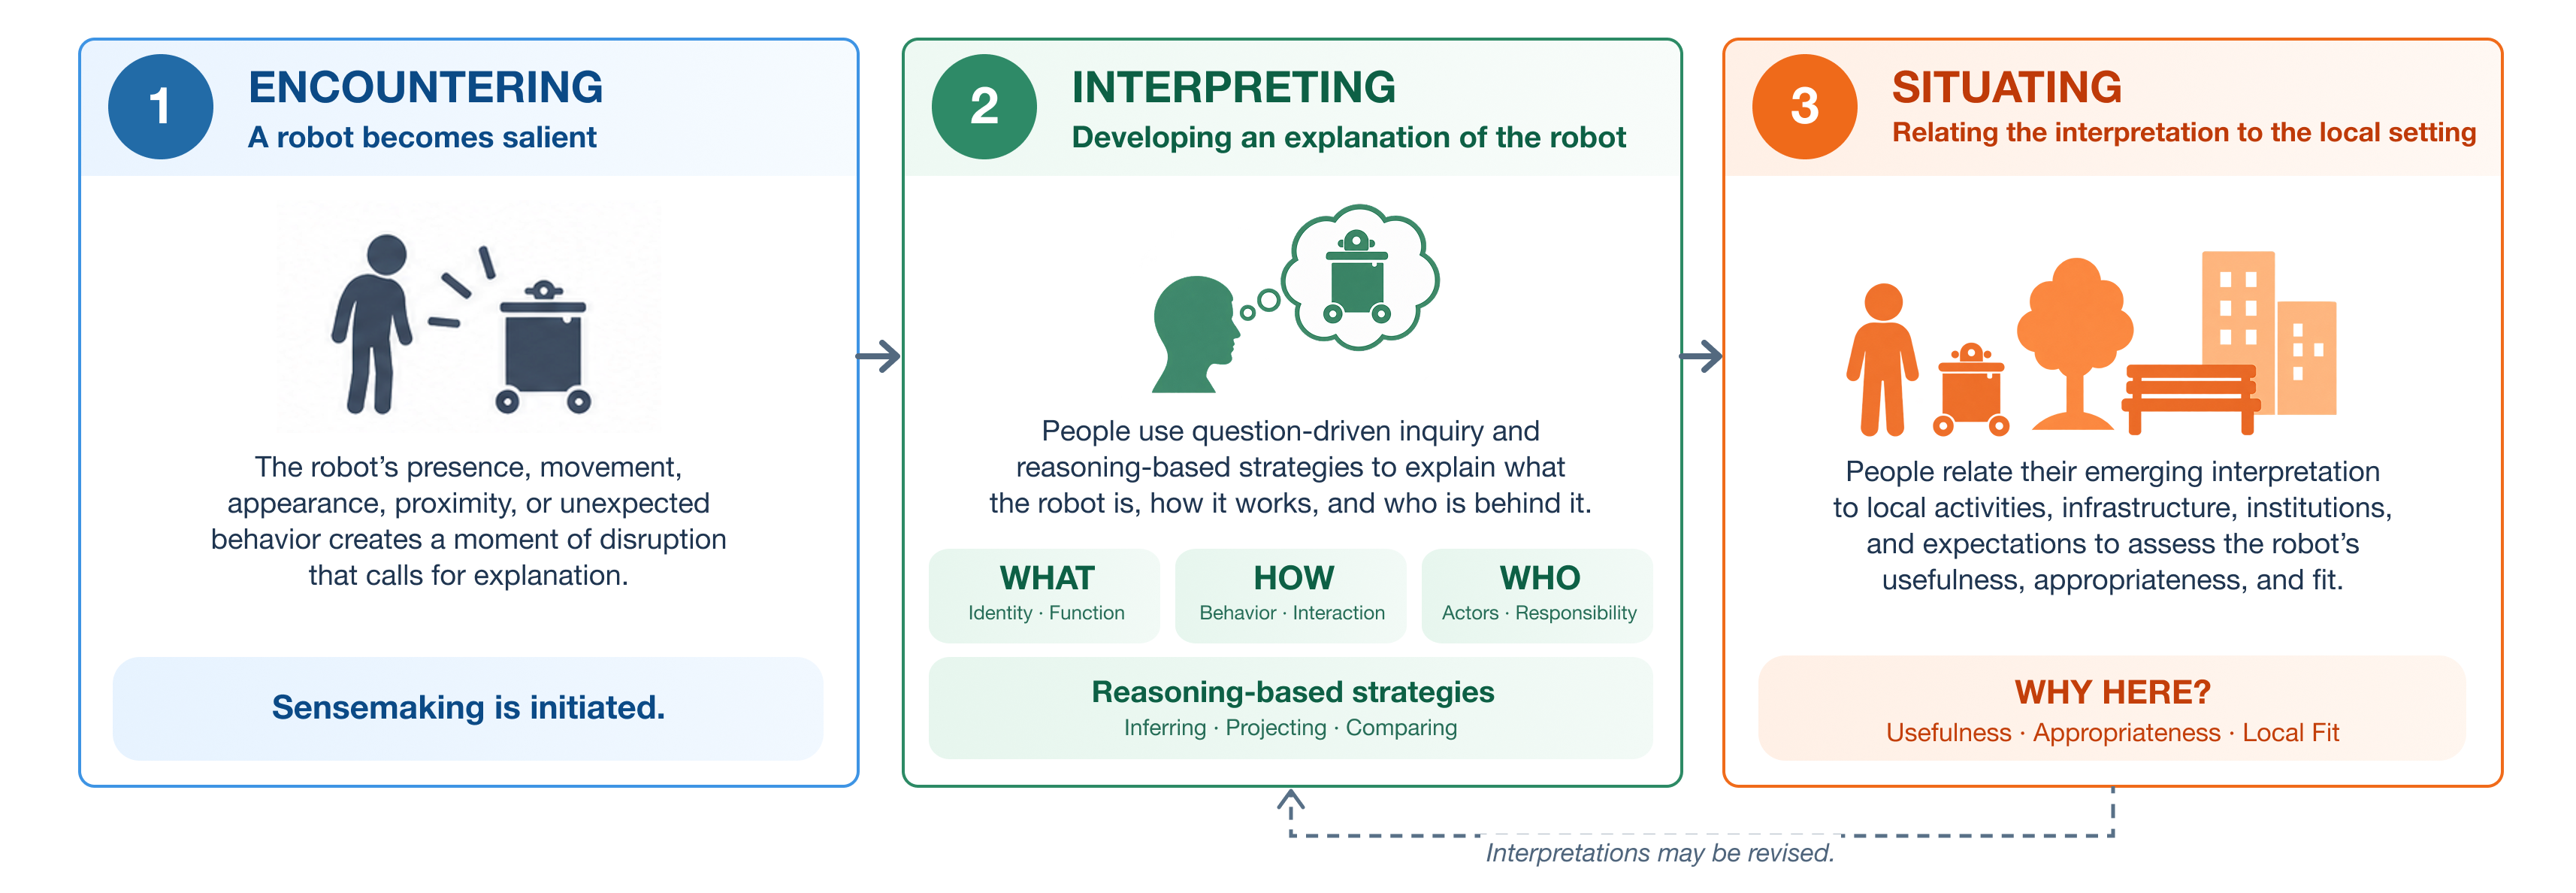
\includegraphics[width=0.95\textwidth]{figures/5.1.png}
    \caption{The interpretive process of public-robot sensemaking.}
    \Description{Conceptual diagram of the interpretive process of public-robot sensemaking, organized into three analytically related components arranged from left to right. The first stage, Encountering, shows a person noticing a robot and describes how the robot's presence, movement, appearance, proximity, or unexpected behavior can make it salient and initiate sensemaking. The second stage, Interpreting, shows people developing an explanation of the robot through question-driven inquiry and reasoning-based strategies. The questions are grouped as WHAT, concerning identity and function; HOW, concerning behavior and interaction; and WHO, concerning actors and responsibility. Reasoning strategies include inference, projection, and comparison. The third stage, Situating, shows people relating their emerging interpretation to local activities, infrastructure, institutions, and expectations in order to assess usefulness, appropriateness, and local fit. A dashed arrow from Situating back to Interpreting indicates that interpretations may be revised.}
    \label{fig:interpretive}
\end{figure*}

Our findings suggest that making sense of a public robot is not an immediate evaluation of whether the robot is useful or acceptable. Rather, it unfolds as an interpretive process through which people first notice the robot, work out what kind of system they are encountering, and then consider what that system means in relation to the place around them. As illustrated in Figure~\ref{fig:interpretive}, we characterize this process as three analytically distinct moments: \emph{encountering}, \emph{interpreting}, and \emph{situating}, a structure that emerged from our analysis and that accordingly organizes how we report the findings. Encountering makes the robot salient as something that calls for explanation; interpreting involves questioning and reasoning through the robot’s identity, operation, and social organization, with recurring concerns around WHAT, HOW, and WHO; and situating relates these emerging interpretation into relation with the local setting, seeking to answer WHY HERE?

This account is consistent with sensemaking as the interpretive work through
which people render an unfamiliar situation intelligible
~\cite{weick2005organizing}.  The Trashbot's familiar trash-can form provided an initial cue, but its movement, camera, proximity, and apparent autonomy made that cue insufficient to explain the system as a whole. This ambiguity exposes interpretive work that is often implicit in public HRI. Prior research has examined different parts of this problem: legibility concerns how observers infer a robot's goals from its behavior~\cite{dragan2013legibility}; mental-model research examines how people form expectations about autonomous systems from incomplete evidence~\cite{paepcke2010judging,riek2012wizard}; field studies show pedestrians working out how to approach, avoid, assist, or coordinate with unfamiliar robots~\cite{pelikan2024encountering,dobrosovestnova2022little,weinberg2023sharing}; and privacy research raises questions about who is sensing, who receives the resulting data, and for what purpose~\cite{denning2014insitu,dietrich2026bystander}.

Seen together, these concerns align with the recurring WHAT, HOW, and WHO questions in our data. WHAT concerns the robot's identity and purpose, extending legibility beyond inferring an immediate motion goal; HOW concerns how its behavior, sensing, and interaction are produced; and WHO locates the robot within a broader socio-technical arrangement of operators, institutions, data recipients, and responsible stakeholders. These questions are especially consequential for bystanders, who encounter robots without prior instruction or an assigned relationship to them~\cite{scholtz2003theory,rosenthal2020forgotten}. Because definitive answers were rarely available, participants worked provisionally: they inferred from visible and behavioral cues, projected possible actions and consequences, and compared the Trashbot with familiar technologies and situations. This resembles the inferential work described in legibility and mental-model research~\cite{dragan2013legibility,paepcke2010judging}, while also drawing on prior experience and shared knowledge~\cite{clark1996using,weick2005organizing}. Questioning and reasoning are therefore complementary: questions identify gaps in an emerging account, while inference, projection, and comparison provide ways of filling them.

Yet resolving WHAT, HOW, and WHO did not settle the encounter. Participants also related these provisional interpretations to the activities, infrastructure, institutions of the surrounding place, echoing prior work showing how robots become embedded within existing workflows, social arrangements, and physical environments ~\cite{mutlu2008robots}. We characterize this as \emph{situating}. WHY HERE? is therefore not simply a fourth question equivalent to WHAT, HOW, and WHO: it asks whether a system understood in those terms makes sense in this particular setting. This move is consistent with situated accounts in which meaning is produced in relation to the circumstances of action~\cite{suchman1987plans}, and with work arguing that public robots must be understood within the particular social organization of the places they enter~\cite{pelikan2025localism,bu2025making}. Public-robot sensemaking thus moves from making the robot intelligible to making its presence locally intelligible, providing the basis for the concept of \emph{local legibility} that we discuss next.

\subsection{Local Legibility as a Basis for Public Robot Interpretation}
\label{sec:local-legibility}

% The findings suggest an extension of legibility as a design concern. 
In HRI, legibility has often referred to whether an observer can infer a robot's immediate goal from its behavior or motion~\cite{dragan2013legibility}. Our findings suggest that, for public service robots, legibility is a basis for the broader interpretive process we discussed in Section~\ref{sec:service-justification}. Participants were not only trying to make sense what the Trashbot was about to do in the moment; they frequently used questioning and reasoning to interpret its broader presence, then situated these interpretation within the local setting. We therefore call a public service robot \emph{locally legible} when people can understand its role within the place where they encounter it. This includes its immediate function and interaction cues, along with the institution responsible for it, the service it provides, the meaning of its sensing or recording, and its relation to existing infrastructure and labor. This extends legibility from a relation between behavior and interpreted goal to a relation among the robot, its broader service arrangement, and the site in which it exists~\cite{while2021urban}.

\paragraph{Accountable attribution} For a public robot to be locally legible, people should be able to identify the stakeholders responsible for its presence and operation. This corresponds to the WHO questions in our findings, through which participants sought to locate the Trashbot within a broader social arrangement. Prior work on privacy-sensitive robotics and bystander privacy has emphasized that public robots affect people who may never choose to interact with them, making questions of who collects, receives, and governs sensed information~\cite{rueben2018themes, dietrich2026bystander}. Dietrich et al., in particular, show how robotic agency can complicate the attribution of actor roles within information flows. In our study, the Campus Café research setting offered participants a plausible institutional attribution, leading them to interpret the Trashbot as a student or research project associated with the surrounding institute. At street and park sites, participants drew on familiar service arrangements, including city sanitation and park management, to infer its affiliation. The responsible institution may need to be identifiable to people who directly interact with the robot, as well as to bystanders who encounter it without choosing to engage. Earlier organizational HRI studies similarly show that robotic services become embedded in existing workflows and relationships beyond the immediate user interaction~\cite{mutlu2008robots,lee2012ripple}. The robot's service role also has to make sense alongside workers and infrastructure already performing related functions. Institutional attribution is therefore part of the public interface: deployments should make clear who is responsible for the robot and how that responsibility relates to the existing division of work and service already in place.

\paragraph{A recognizable local need} 
Local legibility also requires that people can understand \textit{why} the robot belongs in the place where they encounter it and what problem its service helps address. Before people can judge whether a robot is needed \emph{here}, they first need to understand what service it provides and how that service works. In our deployments, confusion was therefore understandable and expected because the Trashbot did not always make its function or intended interaction apparent on its own. Our participants then drew on situated knowledge of the surrounding infrastructure, activities, and local norms to judge whether that service made sense in the site. The same mobile trash service could appear useful where receptacles were distant or poorly maintained, yet unnecessary where fixed bins and cleaners already provided adequate sanitation in the space. Participants also drew on their familiarity with local norms and expected reactions of others to judge whether the Trashbot would be accepted, respected, and used as intended, and thus whether its service could realistically work in that site. This aligns with prior work on localism in public robot design, which argues that public space is not a uniform setting but is organized through site-specific activities, norms, and social relations~\cite{pelikan2025localism}. Related field studies likewise show how cultural knowledge, communal common ground, and everyday activity shape the interpretation of robots in public settings~\cite{bu2025making}. Our findings extend this work by showing how people use such situated knowledge to assess both the need for a robot's service and whether that service can plausibly become part of the setting. A robot's presence may therefore become easier to make sense of when its features and behavior, together with cues from the surrounding environment, point to a recognizable local problem and a role that people can see working there.

\paragraph{Accommodating individual differences} 
Local legibility is also shaped by differences among the people who share a place and should not imply that a place has one single shared interpretation of a public robot. Even within the same site, our participants drew on different prior experiences, associations, and expectations when making sense of the Trashbot. Associations with benevolent or threatening fictional robots, for example, contributed to contrasting interpretations, while recording practices that seemed acceptable to some participants and raised concerns for others. Prior work has documented the cultural and experiential resources people draw on when interpreting public robots~\cite{bu2025making}, as well as variation in how bystanders respond to recording technologies in public settings~\cite{denning2014insitu}. Our findings bring these perspectives into account of local legibility by showing that shared exposure to the same local infrastructure, practices, and robot does not guarantee a shared interpretation. Adapting a robot to a site's infrastructure and practices may still leave individual concerns unresolved. Therefore, local legibility should be treated as an ongoing process of explanation and adjustment. Alongside making the robot's purpose and recording practices explicit, deployments could offer ways to request further information, decline interaction, and communicate concerns that inform changes to robot behavior or operating practices. These mechanisms would help deployments respond to the different people who share a place.

\subsection{Design Implications for Locally Legible Deployment} 
\label{sec:deployment-relationship} 
Building on the three factors underlying local legibility discussed in Section~\ref{sec:local-legibility}, we propose three corresponding design implications: make the institution identifiable, engage with the community, and disclose sensing and data practices. We address these implications in the same order, translating each factor into actionable guidance for designing and operating public robots.

\paragraph{Make the institution identifiable} Prior work has recommended signage and messaging that explain who owns and services public robots~\cite{bu2025making}. Our findings suggest that the design of this information should account for the institutional cues already available at each deployment site. To support accountable attribution as a dimension of local legibility, we recommend placing clearly visible institutional identification on the robot or nearby that is explicitly associated with it. At sites with a recognizable institutional affiliation, such as a university campus, a familiar logo accompanied by a brief statement of the institution's role may help confirm people's understanding of who is responsible for the robot. At sites where this affiliation is less apparent, signage should provide more explicit information about the organization operating the robot, its responsibilities, and whom people can contact with questions or concerns. Visible staff could supplement this information by explaining the deployment and clarifying responsibility. Deployment teams should assess whether these cues allow people unfamiliar with the project to identify the responsible institution.

\paragraph{Engage with the community} 
Community engagement should help establish a locally recognizable role for the robot. Our findings show that participants evaluated the Trashbot through their knowledge of existing services and everyday activities. In Little Italy, participants' familiarity with daily cleaning raised questions about the Trashbot's need and additional value to the community, while participants at Astoria Park identified the Trashbot potential uses to fix the site's lack of trash barrels issue. These accounts suggest that local legibility depends partly on whether the robot's placement and operation communicate a purpose that makes sense locally. Building on prior work on co-designing public robots and situated community engagement~\cite{han2024codesign,yavoayalon2023cxr}, we suggest combining site walkthroughs with discussions of proposed deployment scenarios. Residents, workers, site managers, and regular users could identify existing service arrangements, periods of unmet need, and activities that robot operation might disrupt. Using maps, demonstrations, or enactments, deployment teams could then invite participants to interpret specific encounters: what would a robot approaching this location appear to be doing, why would its presence make sense here, and how would it affect the people already using or maintaining the space? These discussions should inform concrete decisions about routes, operating hours, approach behavior, and the division of work between the robot and existing service providers. 

\paragraph{Make sensing and data practices visible} 
Local legibility requires more than disclosing of what a robot is sensing or recording. People should also be able to understand what is collected, why it is collected, who can access it, and how concerns about those practices can be raised. Prior work has highlighted bystander privacy challenges and the need to accommodate changing privacy preferences~\cite{rueben2018themes, dietrich2026bystander}. To support local legibility, we recommend pairing visible explanations of sensing practices with a clearly advertised channel for questions and feedback throughout a deployment. This channel could include contact information on the robot or nearby signage, a feedback form, and opportunities to speak with deployment team. It should support both individual and community-level concerns.  At the individual level, people should be able to request clarification, raise concerns about a particular encounter, or communicate that they do not wish to be recorded. The team should explain how these requests will be handled and communicate any resulting changes. At the community level, recurring concerns could inform changes to sensing coverage, recording schedules, or data access. Maintaining this exchange would allow both privacy practices and their explanations to remain responsive to the people who encounter the robot.